LZ will use an Optical Calibration System (OCS) to monitor the performance of the OD. Light will be injected into the OD using an LED-driven system with 30 duplex optical fibres mounted within the array of PMTs and 5 duplex optical fibres mounted beneath the tanks. The injection points situated within the array will maintain calibration of PMTs and monitor their performance. The light transmission of the acrylic tanks will be monitored by the 5 bottom injection points. A schematic illustrating the locations of some of the inject points can be seen in figure \ref{fig:inject}. The OCS will have the capability to inject light from a threshold of $\approx 100 keV_{ee}$ up to $\sim 10 MeV_{ee}$, this range will account the signals produced by neutron capture within the scintillator as well as the large signals from penetrating cosmic muons \cite{LZTDR}. Gain drift of the OD PMTs will be monitored injecting a set number of photons during each calibration and measuring the light collection at each PMT. The gain of the PMTs will be adjusted to ensure consistent light collection throughout the running of the experiment.

\begin{figure}[h!]
    \centering
    \includegraphics[width=0.7\textwidth]{Figures/OD_CUT_THROUGH.png}
    \caption{A schematic of a cut through of the OD were some of the injection points are highlighted in red. Each injection point located at the centre of 4 PMTs.}
    \label{fig:inject}
\end{figure}

\section{System requirements}\label{list:SystemReq}
The requirements for the OCS outlined in the main LZ requirements document are;
\begin{itemize}
    \item Number of photons per CH, 700-50 k photons.
    \item Number of photons globally, 1 M photons.
    \item Pulse variation at level of statistical variation in the OD.
    \item Variation calibration to calibration $< \sim100$ photons at 150 keV.
    \item Calibration steps: 700 - 1200 photons: 100 photons step; 5 - 10k: 1k step.
    \item Pulse width, $< 20$ ns.
    \item Pulsing frequency up to 10 kHz.
    \item Light pulse wavelength: 430-450 nm, 450-460 nm, 365-390 nm.
    \item Alignment, $<5\deg$ misalignment.
\end{itemize}

\section{System overview}
The OCS electronics system consists of 5 Optical Calibration Cards (OCC). Each card consists of a FPGA motherboard, which houses 8 LED pulser boards as well as 2 photo-diode read-back boards. Light from the LED's is fed to the front panel and a photo-diode via a 3-way optical coupler. The components of a OCC can be seen in figure \ref{fig:OCC}. The electronics system for the OCS will interface will the detector via 40 duplex optical fibres which will enter the water tank via an air tight and light tight feed-through port on the top of the tank. The light produced by the system will be monitored by two methods, firstly by two four-channel photo-diode daughter boards controlled by the FPGA board and secondly by a rack mounted calibration PMT (identical to the Hamamatsu R5912 PMTs used in the Outer Detector).

\begin{figure}[h]
    \centering
    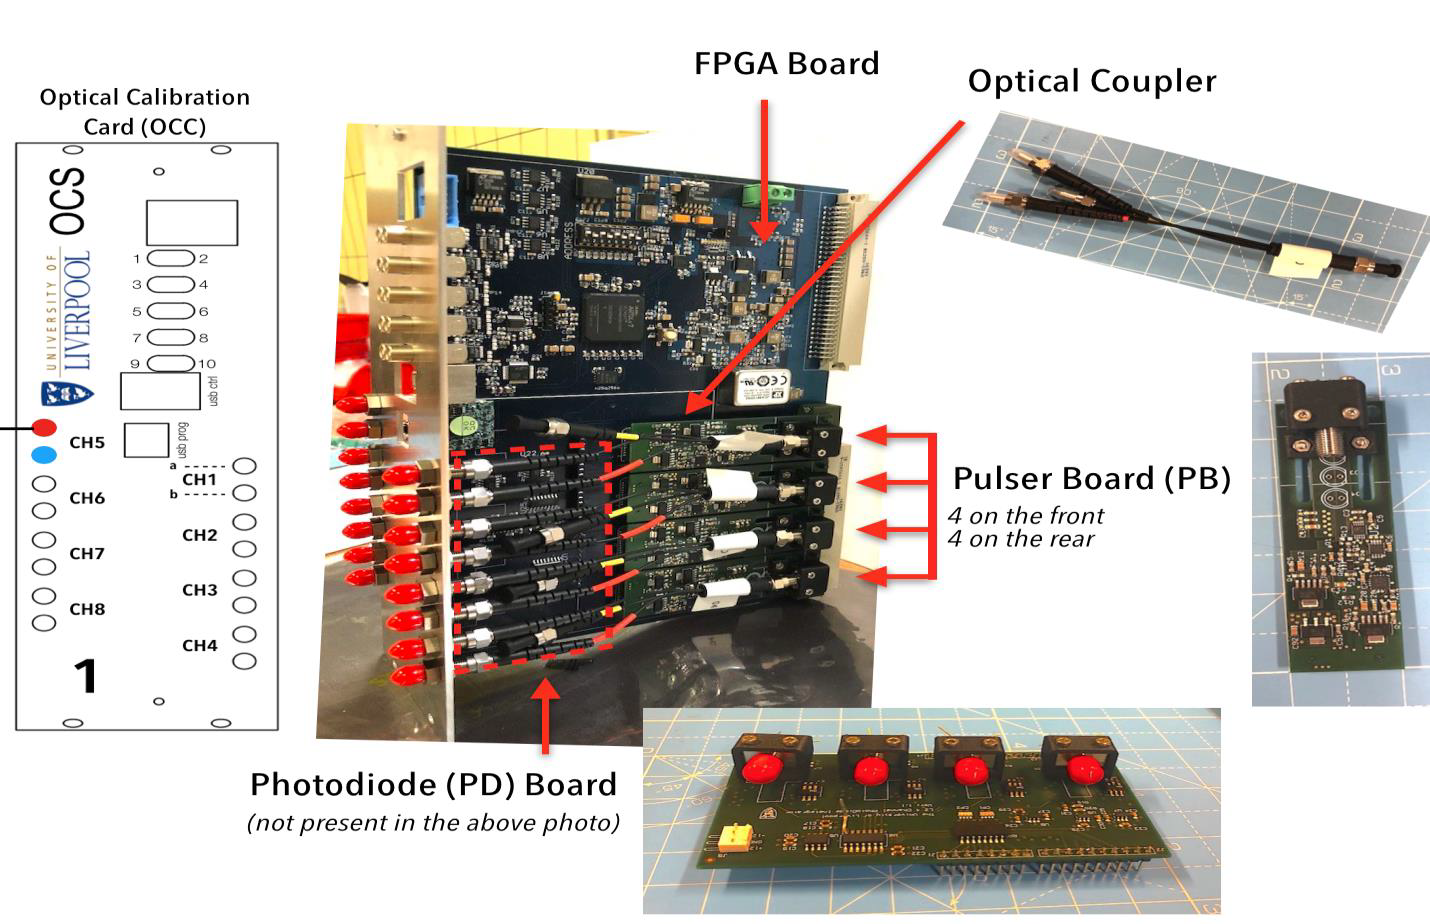
\includegraphics[width=\textwidth]{Figures/OCC.png}
    \caption{From left to right: a diagram of the front panel used on the OCC; a side profile of the FPGA motherboard with pulser boards, photo-diode board and optical couplers labelled respectively.}
    \label{fig:OCC}
\end{figure}

An optical calibration will be initiated by Run Control sending the required pulse configuration to Slow Control. Slow Control will store and manage the data needed to run a calibration. After each calibration run, collected data will be checked against previous calibration run data to ensure consistency of results between runs. The Slow Control system will run using the service, Ignition \cite{IgnitionWeb}, which will display data about the experiment running conditions, manage the database systems and control systems.
\newline
From Slow Control, control commands will pass to a BeagleBone X15 which will communicate with the FPGA boards setting the required registers. The BeagleBone will also read back board temperatures, photo-diode read back, pulse width and LED voltage to the Slow Control for real-time monitoring during calibration runs. A schematic of the OCS can be seen in figure \ref{fig:OCS_Flow}.  

\begin{figure}[ht]
    \centering
    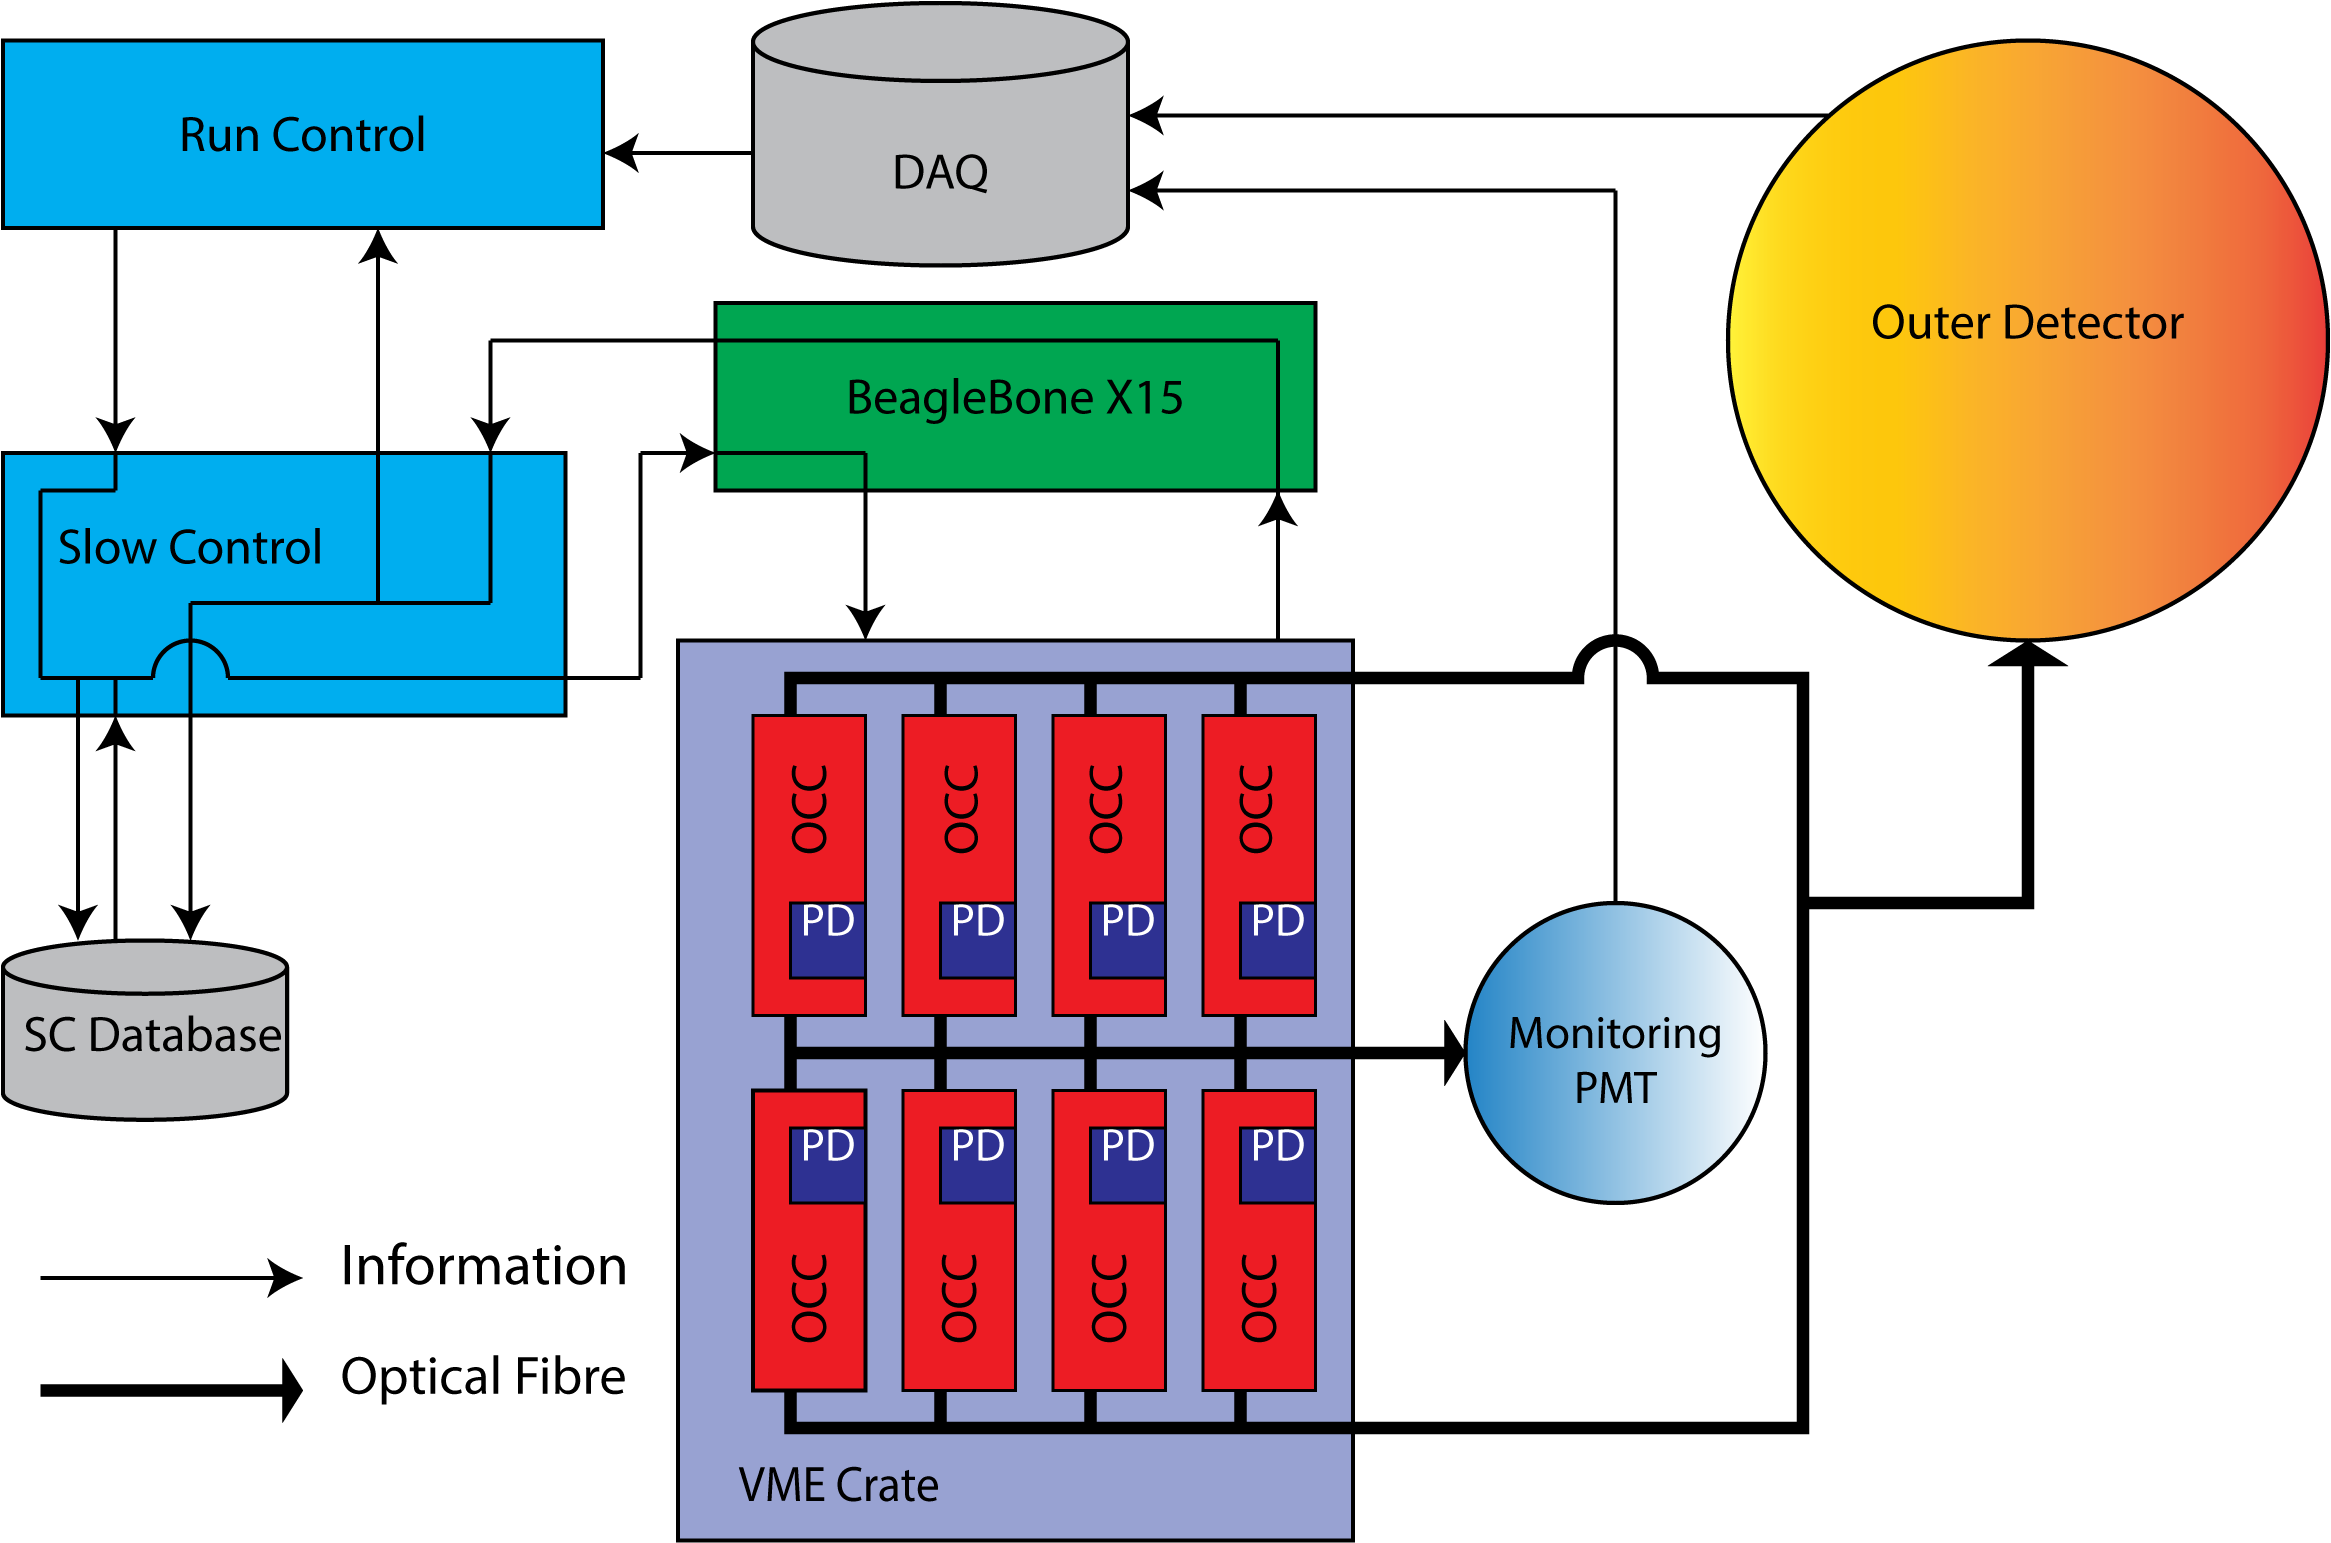
\includegraphics[width=\textwidth]{Figures/OCS.png}
    \caption{A schematic showing the working order in which an Outer Detector Optical Calibration will be completed: RC requests an Optical Calibration of the OD with the required pulse configuration; Slow Control analyses the received pulse configuration and retrieves specific parameters from the Slow Control-Database; Slow Control sends the specific parameters to a BeagleBone-X15; The BeagleBone-X15 communicates the specific commands to the VME Crate/OCCs setting the required registers; Light is pulsed into the OD and monitoring PMT; Readout from the monitoring PMT and OD is sent to the DAQ; Readouts from the photo-diode boards and OCCs are sent back to Slow Control-Database and Run Control via the BeagleBone-X15.}
    \label{fig:OCS_Flow}
\end{figure}